\section{Fitting Data}

\subsection{Task A}

\begin{align*}
    \mu_1 &= \frac{\sum x_i}{N} = 6.50 \\
    \mu_2 &= \frac{\sum x_i^2}{N} = 46.55 \\
\end{align*}

\subsection{Task B}

The histogram of the data is shown in Figure \ref{fig:q3_hist}.

\begin{figure}[H]
    \centering
    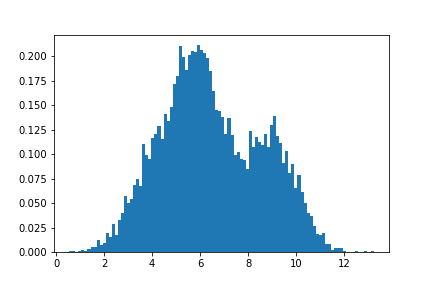
\includegraphics[width=0.7\textwidth]{images/3b.png}
    \caption{Histogram of the data}
    \label{fig:q3_hist}
\end{figure}

\subsection{Task C}

The binomial distribution is given by

\begin{align*}
    \mu_1^{Bin} &= \sum_{r=0}^{n} \binom{n}{r}p^r (1-p)^{n-r} r\\
    &= np\\
    \mu_2^{Bin} &= \sum_{r=0}^{n} \binom{n}{r}p^r (1-p)^{n-r} r^2\\
    &= np\sum_{r=1}^{n} \binom{n-1}{r-1}p^{r-1} (1-p)^{n-r} r\\
    &= np\sum_{r=0}^{n-1} \binom{n-1}{r}p^{r} (1-p)^{n-r-1} (r+1)\\
    &= n(n-1)p^2 + np\sum_{r=0}^{n-1} \binom{n-1}{r}p^{r} (1-p)^{n-r-1}\\
    &= n(n-1)p^2 + np
\end{align*}
The values of $\mu_1^{Bin}$ and $\mu_2^{Bin}$ are 6.50 and 46.55 respectively. These values are the same as the values of $\mu_1$ and $\mu_2$ calculated in Task A.

When the values of $n$ and $p$ are fit the the data and the integers next to $n$ are taken, the values of $n$ and $p$ are 20 and 0.33 respectively.

The histogram of the data and the binomial distribution with $n=20$ and $p=0.33$ is shown in Figure \ref{fig:q3_hist_bin}.

\begin{figure}[H]
    \centering
    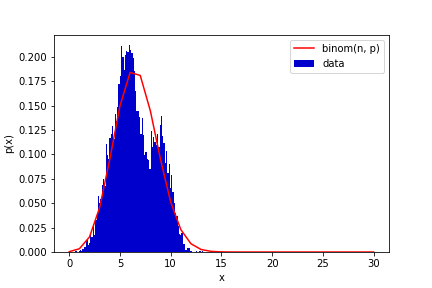
\includegraphics[width=0.7\textwidth]{images/3c.png}
    \caption{Histogram of the data and the binomial distribution with $n=20$ and $p=0.33$}
    \label{fig:q3_hist_bin}
\end{figure}

\subsection{Task D}

The gamma distribution is given by

\begin{align*}
    \mu_1^{Gamma} &= \int_0^\infty f(x;k,\theta)xdx \\
    &= \int_0^\infty \frac{1}{\theta^k \Gamma(k)} x^{k-1} e^{-\frac{x}{\theta}}xdx \\
    &= \frac{\theta^{k+1}\Gamma(k+1)}{\theta^k\Gamma(k)} \\
    &= k\theta 
\end{align*}

\begin{align*}
    \mu_2^{Gamma} &= \int_0^\infty f(x;k,\theta)x^2dx \\
    &= \int_0^\infty \frac{1}{\theta^k \Gamma(k)} x^{k} e^{-\frac{x}{\theta}}xdx \\
    &= \frac{\theta^{k+2}\Gamma(k+2)}{\theta^k\Gamma(k)} \\
    &= k(k+1)\theta^2
\end{align*}

The values of $\mu_1^{Gamma}$ and $\mu_2^{Gamma}$ are 6.50 and 46.55 respectively. These values are the same as the values of $\mu_1$ and $\mu_2$ calculated in Task A.

When the values of $k$ and $\theta$ are fit the the data, the values of $k$ and $\theta$ are 9.70 and 0.67 respectively.

The histogram of the data and the gamma distribution with $k=9.70$ and $\theta=0.67$ is shown in Figure \ref{fig:q3_hist_gamma}.

\begin{figure}[H]
    \centering
    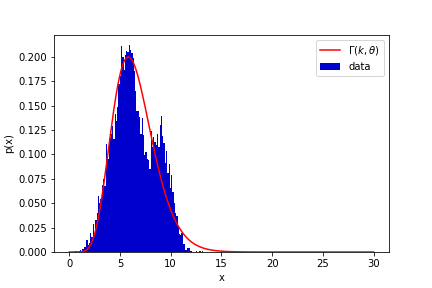
\includegraphics[width=0.7\textwidth]{images/3d.png}
    \caption{Histogram of the data and the gamma distribution with $k=9.70$ and $\theta=0.67$}
    \label{fig:q3_hist_gamma}
\end{figure}

\subsection{Task E}

\textbf{Definition:} \textit{Likelihood} \\
    Given a dataset $S$ and a choice of parameter $\lambda = \lambda_0$ for a family of distributions $P[\lambda]$ parameterized by $\lambda$, define the likelihood of $\lambda_0$ by
    \begin{equation*}
        \mathcal{L}(\lambda_0 \mid S) = P_{\lambda_0}[S] = \prod_{i=1}^{N} P_{\lambda_0}[x_i]
    \end{equation*}

For large datasets, since each probability is a small number, the likelihood can underflow. Thus, the average log-likelihood is typically calculated:

\begin{equation*}
    \ell(\theta \mid S) = \frac{\log \mathcal{L}(\theta \mid S)}{N}
\end{equation*}

The average log-likelihood of the data under the binomial and gamma distributions are -2.157 and -2.161 respectively. Binomial distribution has a higher average log-likelihood than the gamma distribution.

\subsection{Task F}

\begin{align*}
    \mu_1^{gmm} &= p_1 \mu_1 + p_2 \mu_2 \\
    \mu_2^{gmm} &= p_1 (\sigma_1^2 + \mu_1^2 ) + p_2 (\sigma_2^2 + \mu_2^2) \\
    \mu_3^{gmm} &= p_1 (\mu_1^3 + 3\mu_1 \sigma_1^2 ) + p_2 (\mu_2^3 + 3\mu_2 \sigma_2^2) \\
    \mu_4^{gmm} &= p_1 (\mu_1^4 + 6\mu_1^2 \sigma_1^2 + 3\sigma_1^4 ) + p_2 (\mu_2^4 + 6\mu_2^2 \sigma_2^2 + 3\sigma_2^4)
\end{align*}

When the values of $\mu_1$, $p_1$, $\mu_2$, and $p_2$ are fit to the data, with $\sigma_1 = \sigma_2 = 1$, the values of are 5.13, 0.61, 8.77, and 0.38 respectively.

The histogram of the data and the GMM with $\mu_1=5.13$, $p_1=0.61$, $\mu_2=8.77$, and $p_2=0.38$ is shown in Figure \ref{fig:q3_hist_gmm}.

\begin{figure}[H]
    \centering
    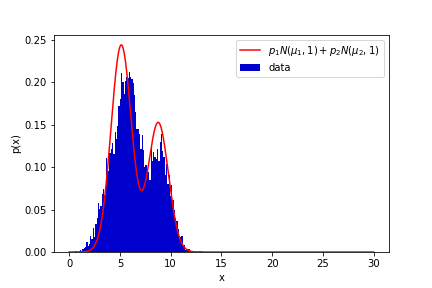
\includegraphics[width=0.7\textwidth]{images/3f.png}
    \caption{Histogram of the data and the GMM with $\mu_1=5.13$, $p_1=0.61$, $\mu_2=8.77$, and $p_2=0.38$}
    \label{fig:q3_hist_gmm}
\end{figure}